\textbf{Цель работы:} измерить энергию первого уровня атома гелия в динамическом и статическом режимах методом электронного возбуждения.

\textbf{Используемое оборудование}: трёхэлектродная лампа ЛМ-2, батарея 4.5 В, микроамперметр, понижающий трансформатор, осциллограф, блок источников питания,вольтметр В7-22А.
             
\section{Теоретическое введение}

    \begin{figure}[!h]
        \centering
        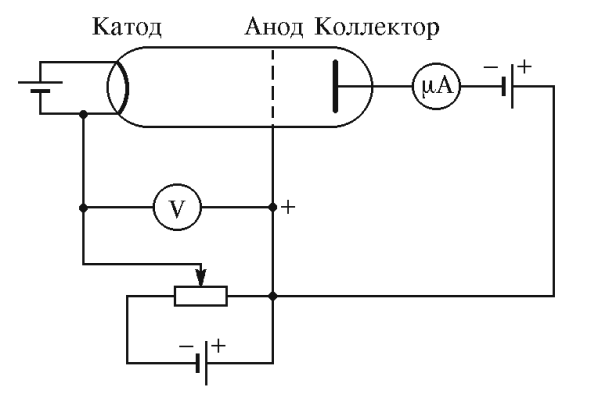
\includegraphics[width = 10 cm]{images/exp_scheme}
        \caption{Схема опыта Франка-Герца}
        \label{fig:vac}
    \end{figure}

    Опыт Франка-Герца подтверждает существование дискретных уровней энергии атомов. Разреженный одноатомный газ заполняет трёхэлектродную лампу. Электроны, испускаемые разогретым катодом, ускоряются в постоянном электрическом поле, созданном между катодом и сетчатым анодом лампы. Передвигаясь от катода к аноду, электроны сталкиваются с атомами гелия.

    При увеличении потенциала анода ток в лампе вначале растет, однако, когда энергия электронов становится достаточной для возбуждения
    атомов, ток коллектора резко уменьшается. Это происходит потому, что при неупругих соударениях с атомами электроны почти полностью теряют свою энергию и не могут преодолеть задерживающего потенциала (около 1 В) между анодом и коллектором. При дальнейшем увеличении потенциала анода ток коллектора вновь возрастает: электроны, испытавшие неупругие соударения, при дальнейшем движении к аноду успевают набрать энергию, достаточную для преодоления задерживающего потенциала.

    Следующее замедление роста тока происходит в момент, когда часть электронов неупруго сталкивается с атомами два раза: первый раз посередине пути, второй -- у анода и т. д.

    \begin{figure}[h!]
        \centering
        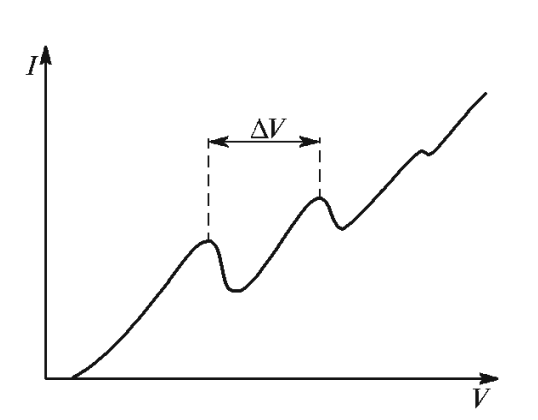
\includegraphics[width = 9 cm]{images/exp_IU_dep}
        \caption{Схематический вид зависимости тока коллектора от напряжения на аноде}
        \label{ris:experimcoded}
    \end{figure}

    Кинетическая энергия электрона 1 уровня равна:
    \begin{equation}
        \label{key}
        E = \overline{e} \Delta V \left[\text{эВ}\right],
    \end{equation}
    где $\Delta V$ -- разность между двумя пиками (см. рис. \ref{ris:experimcoded}).
   
\section{Экспериментальная установка}

    На рис. \ref{fig:vac} обозначены: $A$ - амперметр; $\text{Б}7-4$ -- стабилизированный источник питания (подаёт напряжение накала); $K_1$ -- тумблер для включения в цепь источника $\text{Б}7-4$; $\text{Б}5-10$ -- выпрямитель (подаёт на анод ускоряющее напряжение); $Pi_3$ - потенциометр, регулирующий величину ускоряющего напряжения; $V_1$ -- вольтметр, измеряющий величину ускоряющего напряжения; 4.5 $B$ -- батарея КБСЛ; $Pi_2$ - потенциометр, регулирующий величину задерживающего потенциала; $V_2$ - вольтметр, измеряющий величину задерживающего потенциала; $\mu A$ - микроамперметр; $K_3$ -- ключ, переключающий схему из статического режима в динамический; Т -- понижающий трансформатор -- подаёт ускоряющий потенциал при динамическом режиме.

    \begin{figure}[!h]
        \centering
        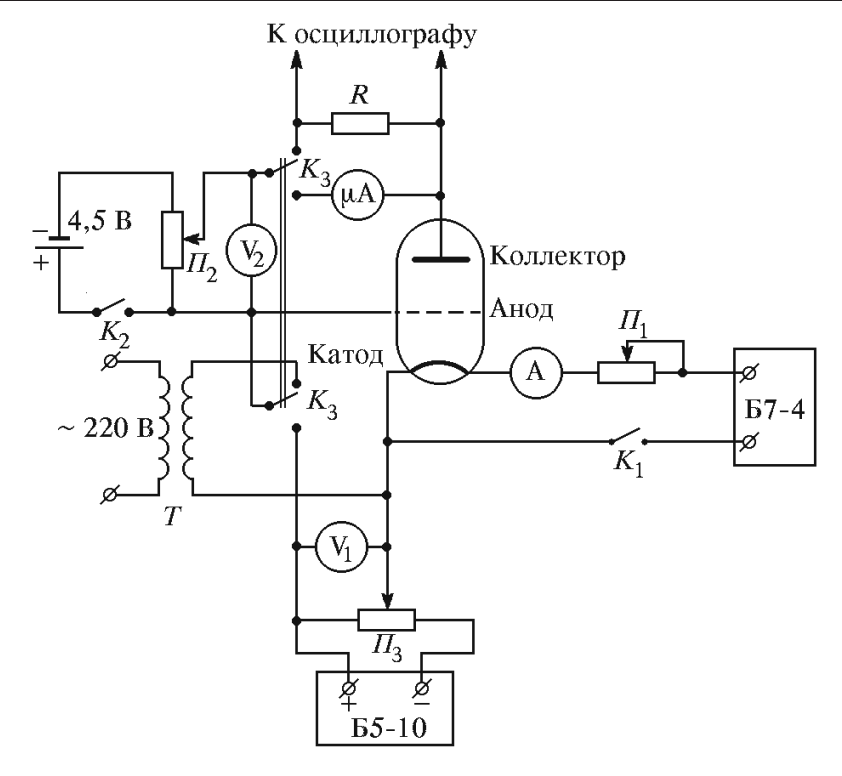
\includegraphics[width = 13 cm]{images/exp_equipment}
        \caption{Схема экспериментальной установки}
        \label{fig:exp_eq}
    \end{figure}
    
\section{Ход работы}

\subsection{Динамический режим измерений}

    С помощью осциллографа снимем осциллограммы зависимости $V_k(V_a)$, затем по осцилограммам определим энергию возбуждения первого уровня атома гелия.

    \begin{figure}[H]
        \centering
        \subfigure{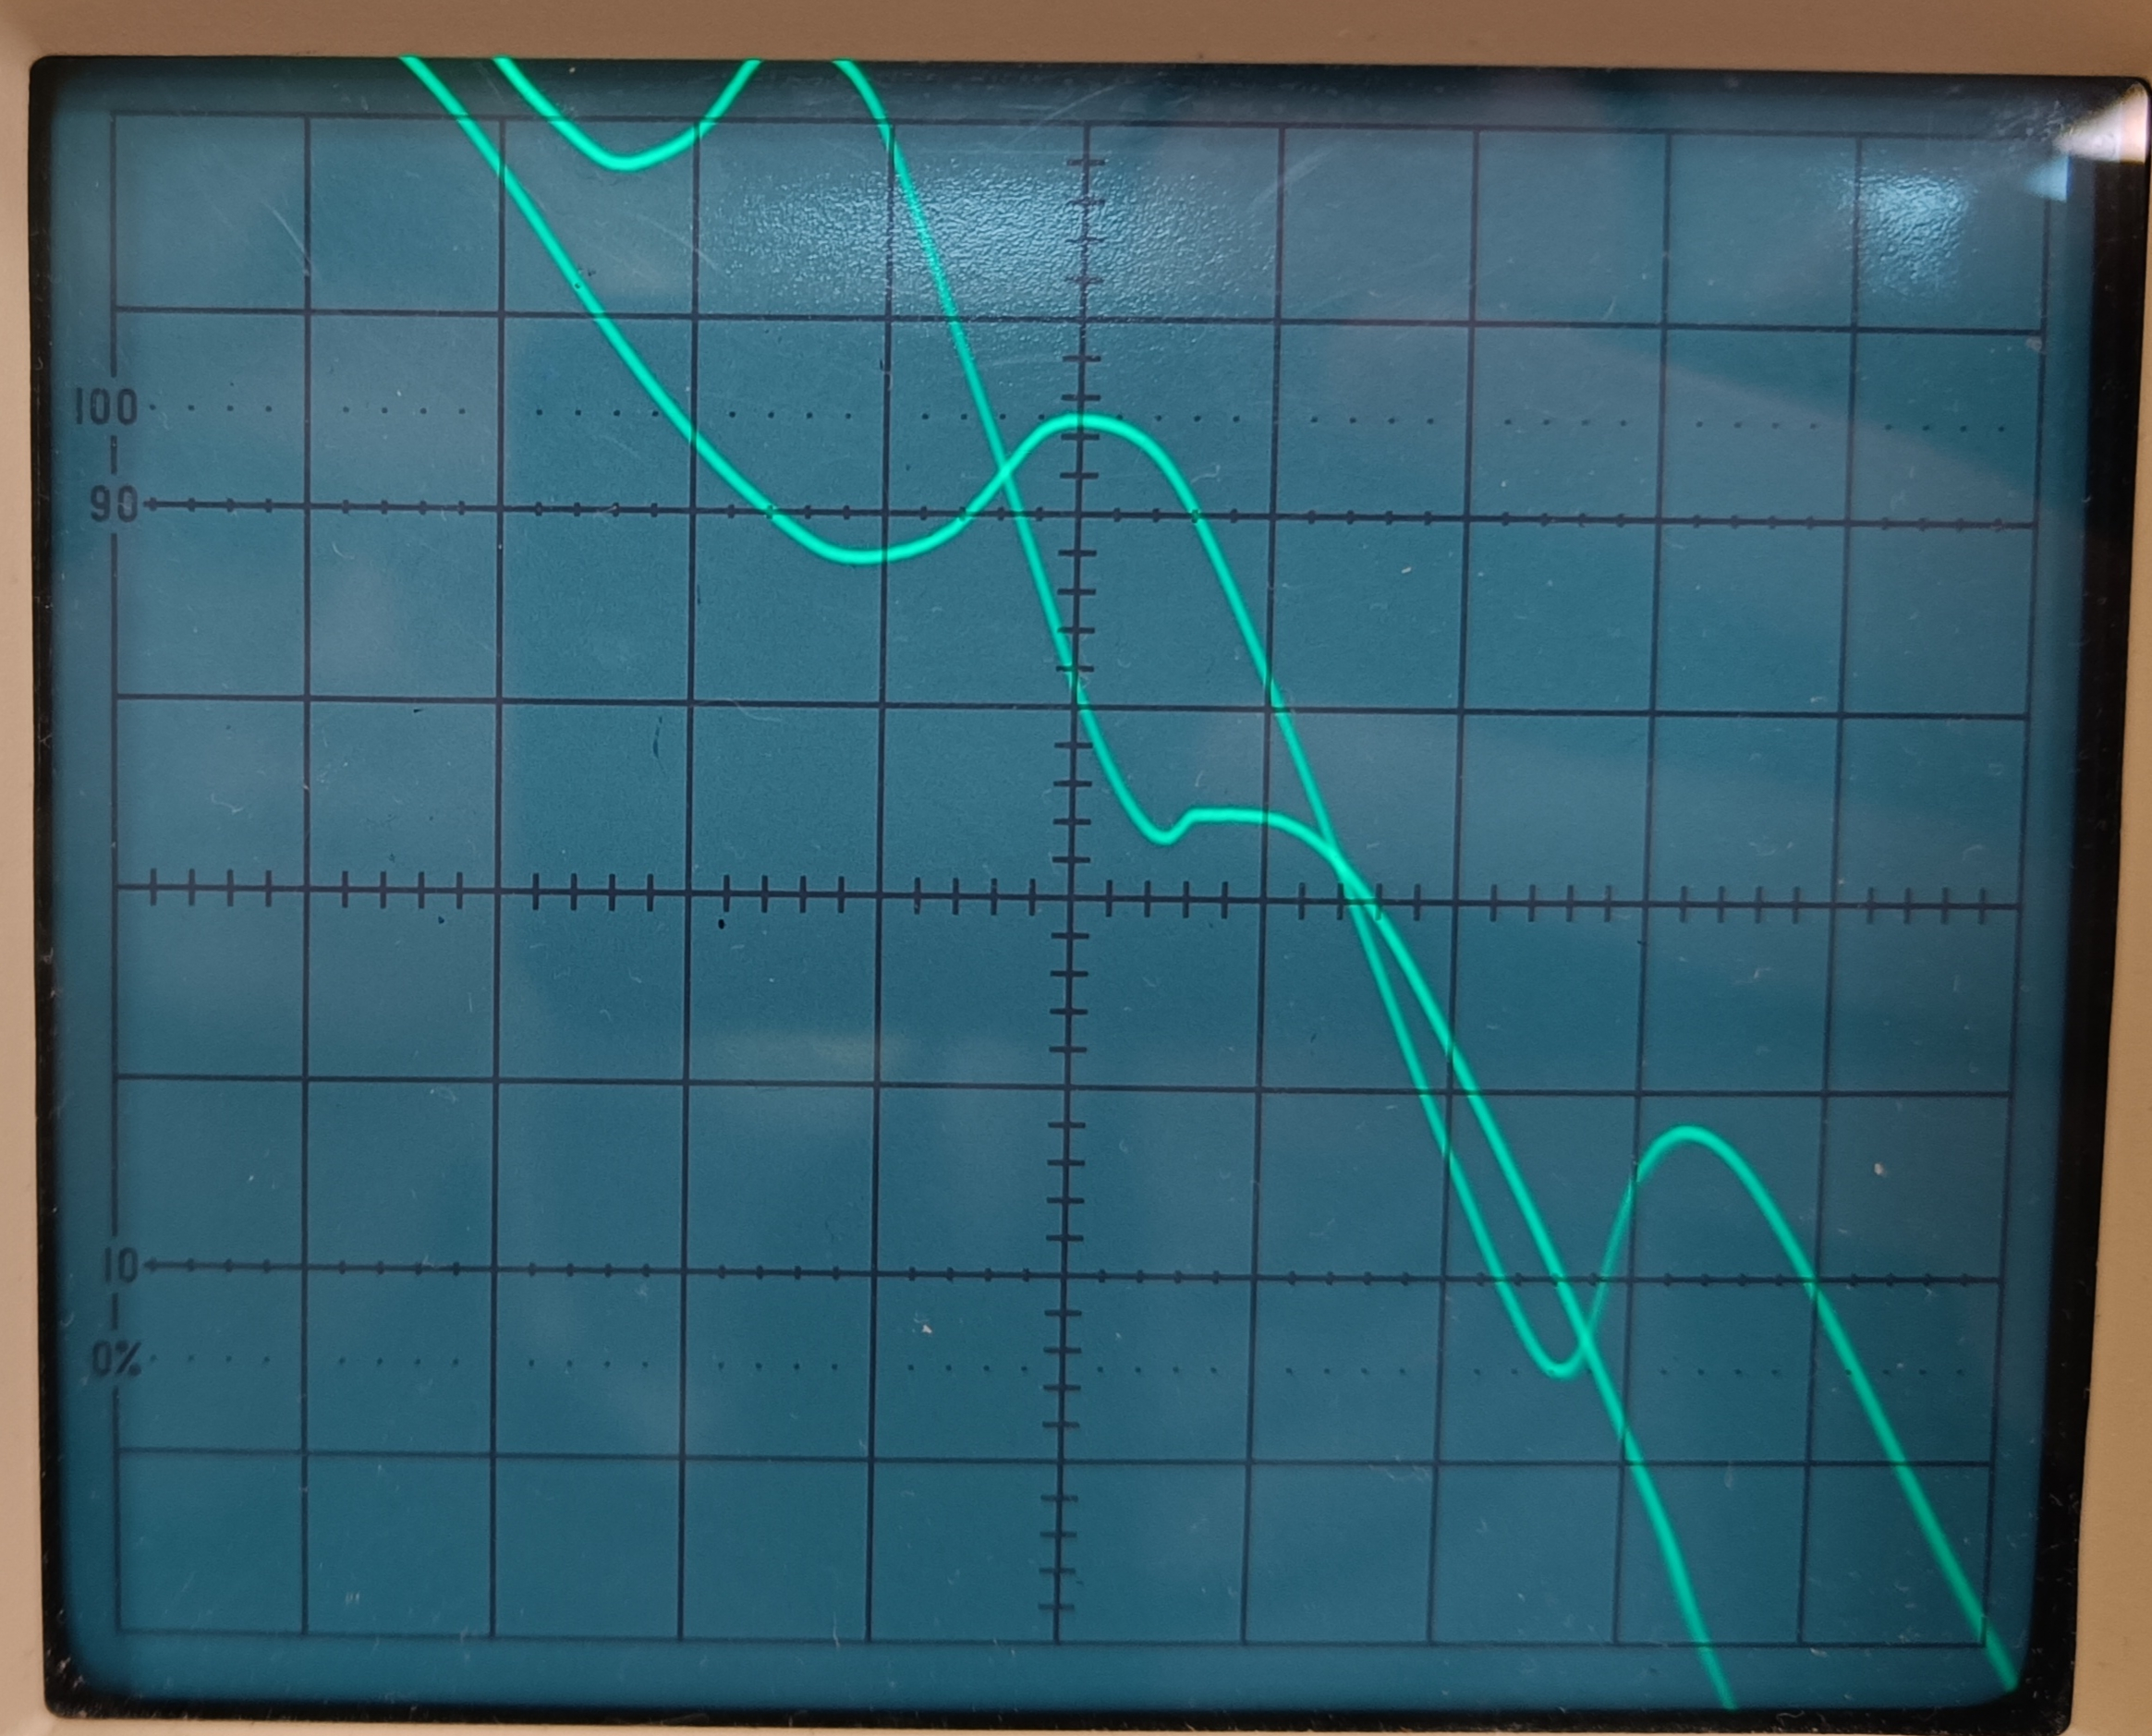
\includegraphics[width=0.48\textwidth]{images/V_th_4_1.jpg}} 
        \subfigure{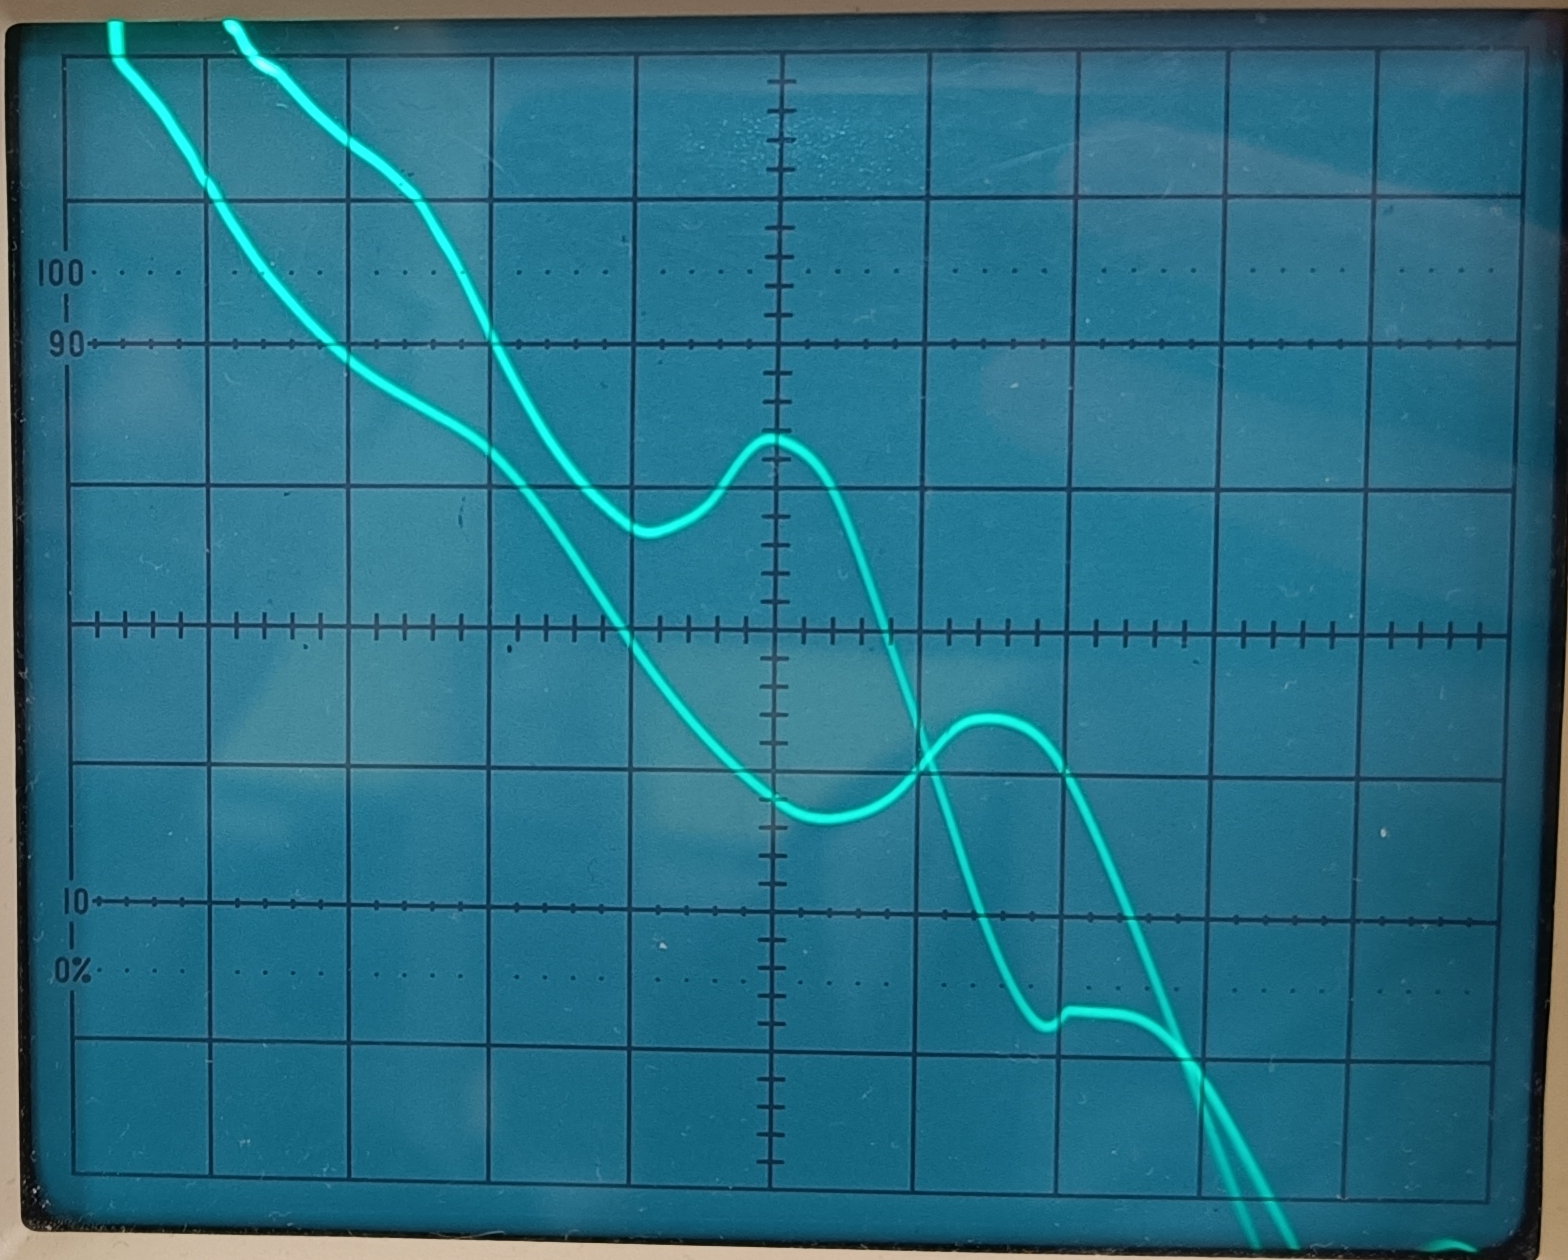
\includegraphics[width=0.48\textwidth]{images/V_th_4_2.jpg}} 
        \caption{Осциллограмма при задерживающем напряжении $V_{\text{зад}} = 4$ В}
        \label{fig:vth4}
    \end{figure}

    \begin{figure}[H]
        \centering
        \subfigure{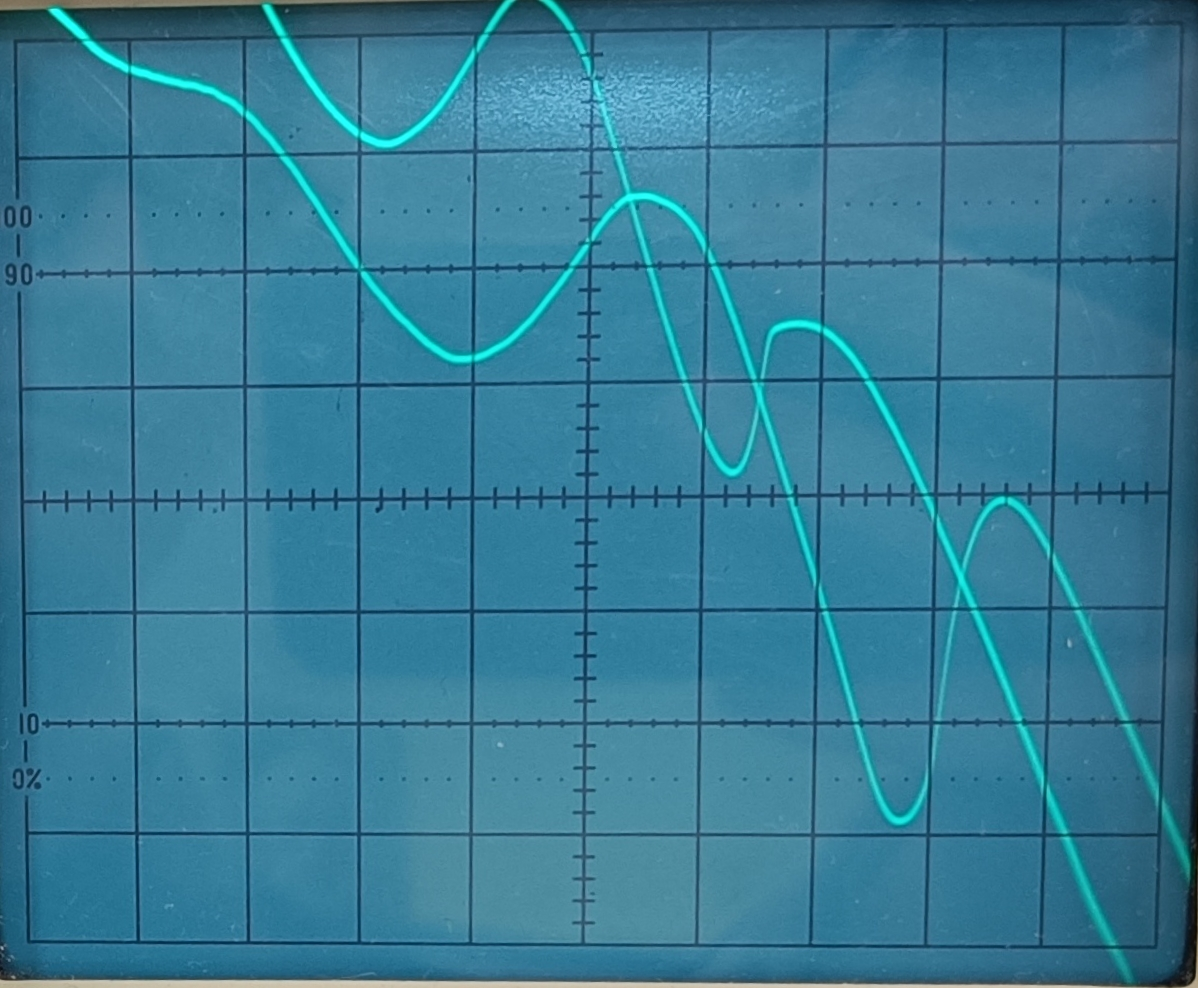
\includegraphics[width=0.48\textwidth]{images/V_th_6_1.jpg}} 
        \subfigure{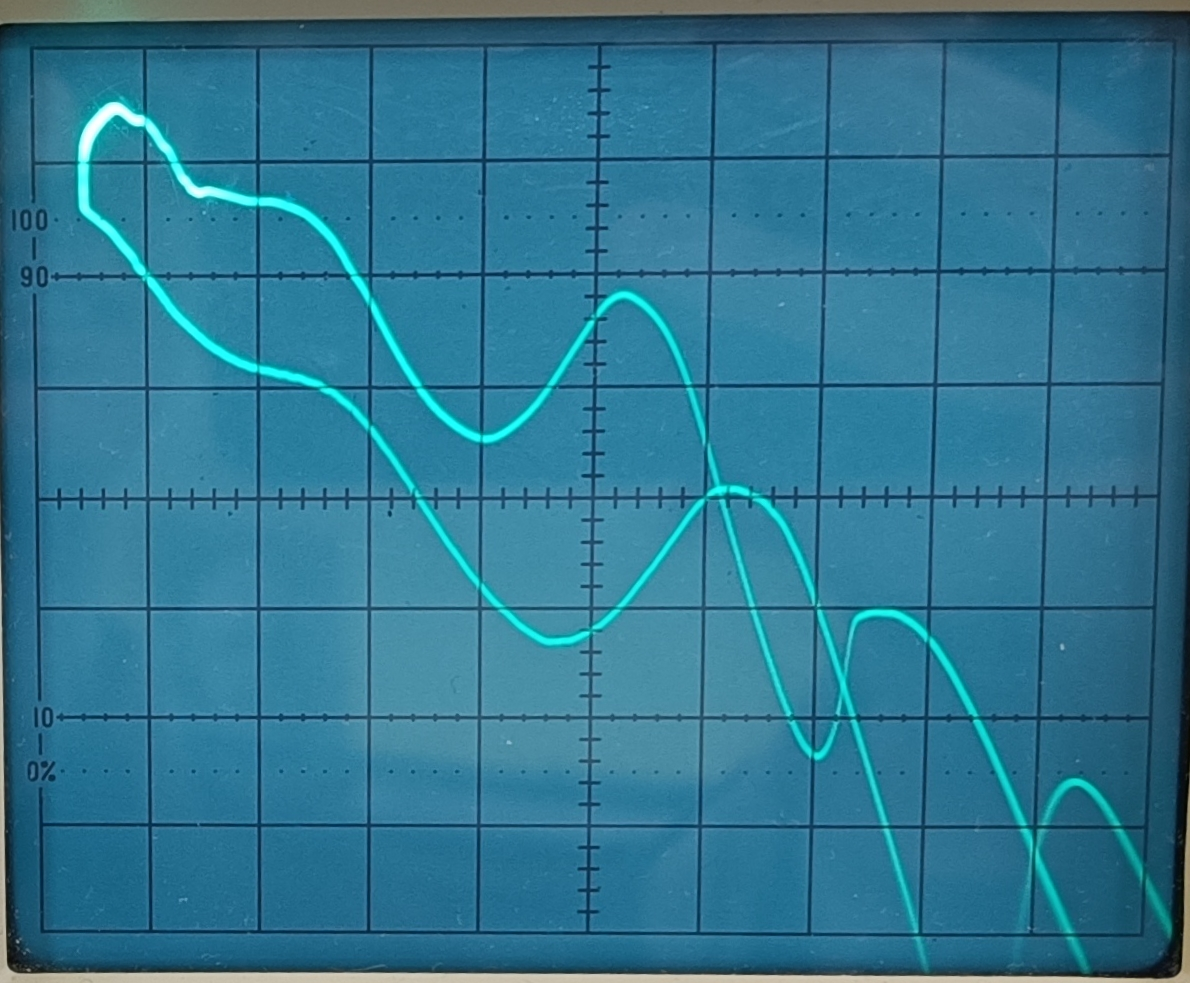
\includegraphics[width=0.48\textwidth]{images/V_th_6_2.jpg}} 
        \caption{Осциллограмма при задерживающем напряжении $V_{\text{зад}} = 6$ В}
        \label{fig:vth6}
    \end{figure}

    \begin{figure}[H]
        \centering
        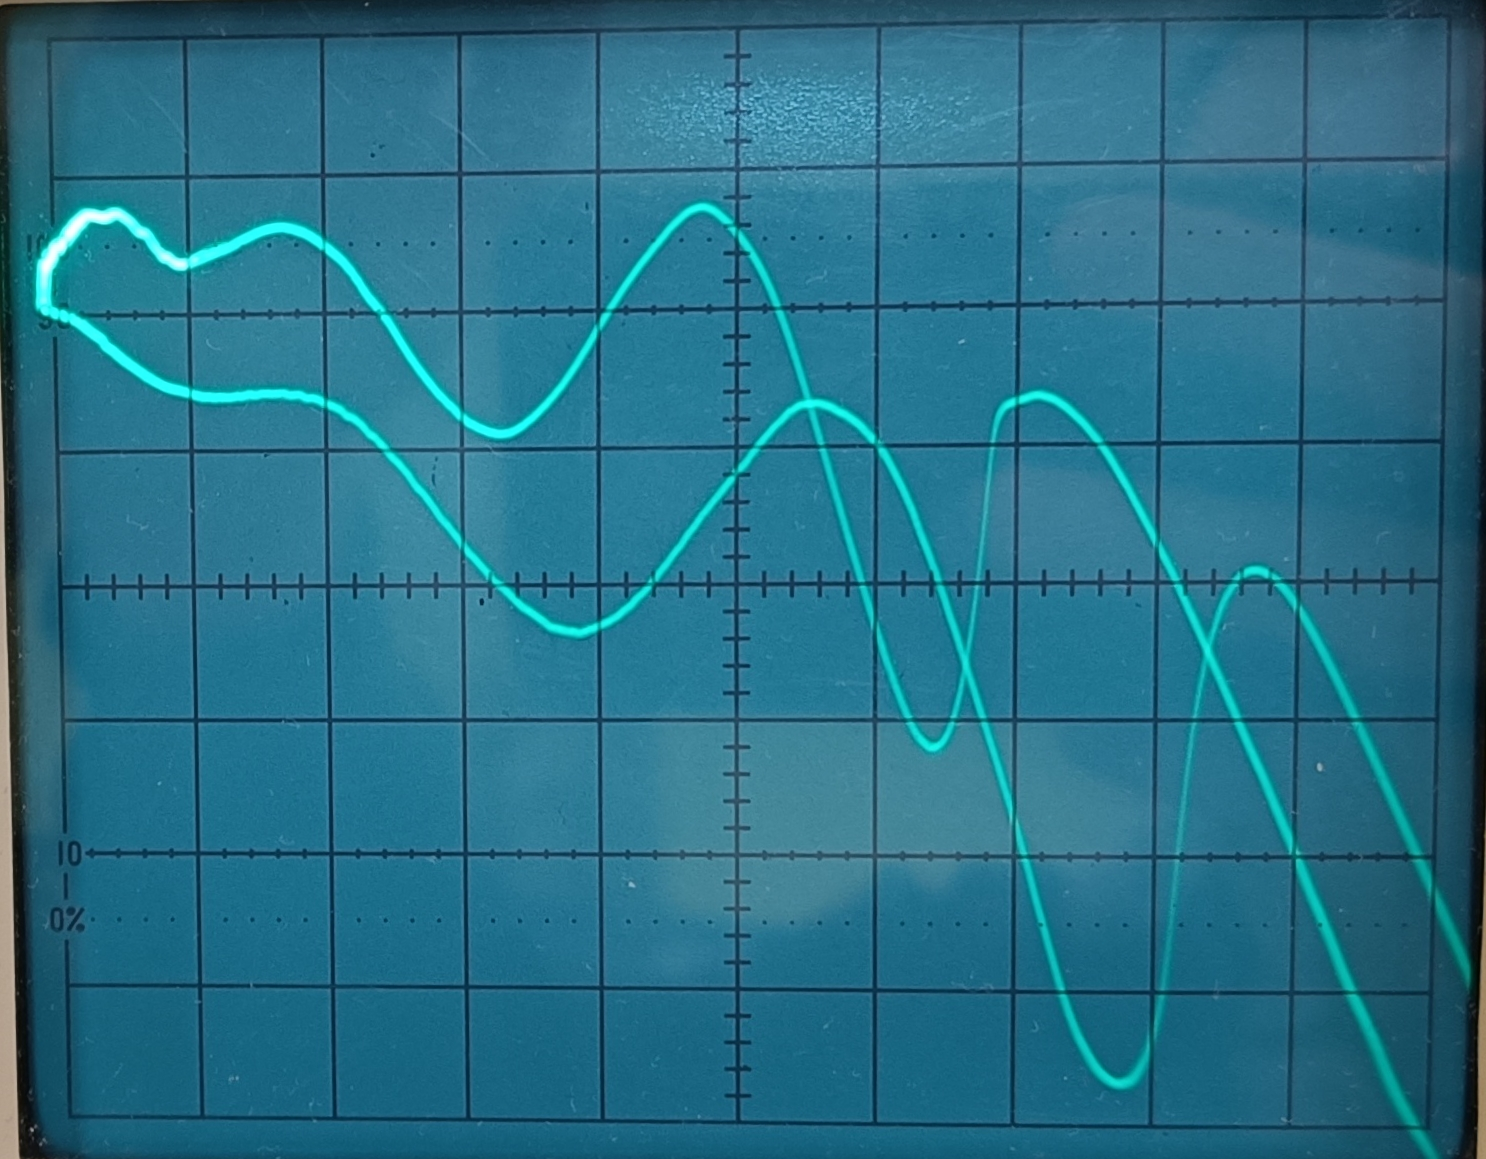
\includegraphics[width=0.59\textwidth]{images/V_th_8_1.jpg}
        \caption{Осциллограмма при задерживающем напряжении $V_{\text{зад}} = 8$ В}
        \label{fig:vth8}
    \end{figure}

    \begin{table}[H]
        \centering
        \begin{tabular}{|c|c|c|c|c|}
            \hline
            $V_{\text{зад}}$ & $\Delta V_{max_1}$ & $\Delta V_{max_2}$ & $\Delta V_{min_1}$ & $\Delta V_{min_2}$ \\ \hline
            4                & 16.5               & 12.5               & 17.5               & 14.5               \\ \hline
            6                & 16                 & 12.5               & 19                 & 15                 \\ \hline
            8                & 15                 & 12.5               & 19.5               & 13.5               \\ \hline
        \end{tabular}
    \end{table}

    Из разностей минимум и максимумов на осциллограмме посчитаем значения энергии возбуждения первого уровня атома гелия (как среднее значение):
    \begin{equation}
        E_d = (15.33 \pm 0.74) \; \text{эВ}
    \end{equation}

\subsection{Статический режим измерений}

    С помощью амперметра и вольтметра снимем зависимость $I_k(V_a)$ при различных задерживающих напряжениях.

    \begin{figure}[H]
        \centering
        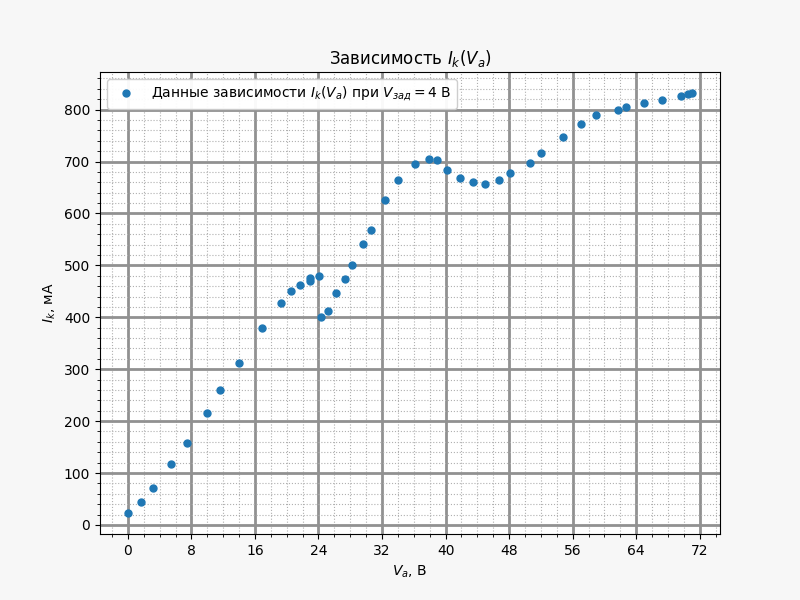
\includegraphics[width = 12 cm]{images/V_th_4_static}
        \caption{График зависимости $I_k(V_a)$ при задерживающем напряжении $V_{\text{зад}} = 4$ В}
        \label{fig:vth4_static}
    \end{figure}

    \begin{figure}[H]
        \centering
        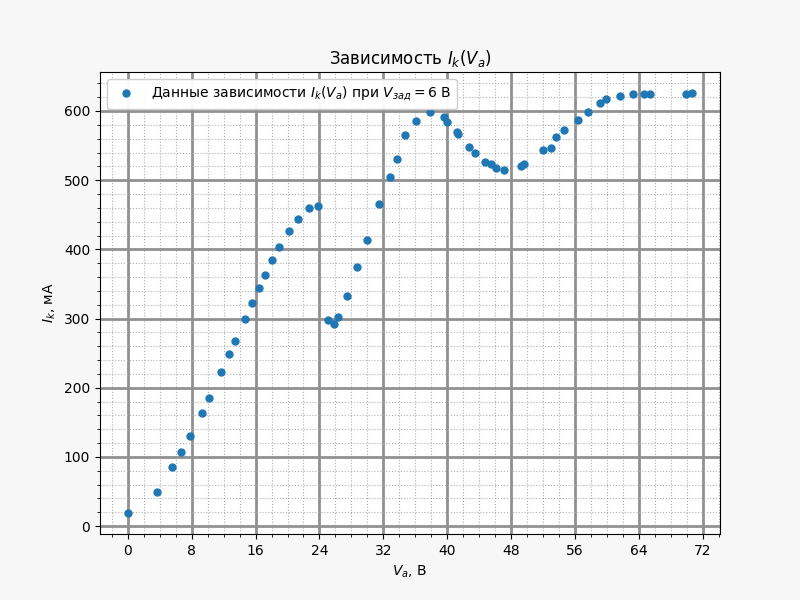
\includegraphics[width = 12 cm]{images/V_th_6_static}
        \caption{График зависимости $I_k(V_a)$ при задерживающем напряжении $V_{\text{зад}} = 6$ В}
        \label{fig:vth6_static}
    \end{figure}

    \begin{figure}[H]
        \centering
        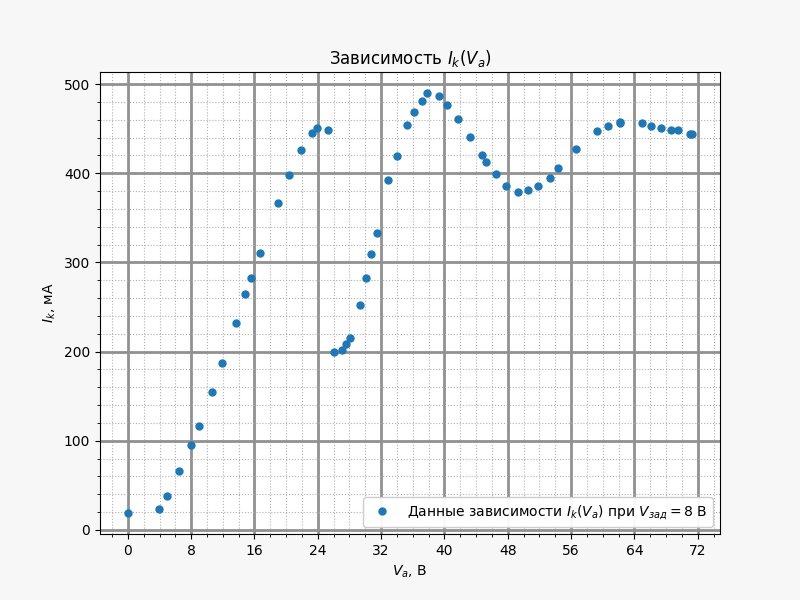
\includegraphics[width = 12 cm]{images/V_th_8_static}
        \caption{График зависимости $I_k(V_a)$ при задерживающем напряжении $V_{\text{зад}} = 8$ В}
        \label{fig:vth8_static}
    \end{figure}

    \begin{table}[H]
        \centering
        \begin{tabular}{|c|c|c|c|c|c|}
            \hline
            $V_{\text{зад}}$ & $\Delta V_{max_1}$ & $\Delta V_{max_2}$ & $\Delta V_{min_1}$ & $\Delta V_{avg}$ & $\sigma_{\Delta V}$\\ \hline
            4                & 14.17              & 26.04              & 20.84              & 20.35            & 3.46                                                           \\ \hline
            6                & 14.13              & 26.11              & 21.88              & 20.71            & 3.48                                                           \\ \hline
            8                & 13.79              & 25.75              & 23.23              & 20.92            & 3.71                                                           \\ \hline
        \end{tabular}
    \end{table}

    Полное усреднение по минимумам и максимум даёт значение энергии возбуждения
    \begin{equation}
        E_{st} = (20.66 \pm 1.78) \; \text{эВ}
    \end{equation}

\section{Заключение}

    В результате эксперимента динамическим режимом измерений с помощью осциллографа получили значение энергии возбуждения первого уровня атома гелия 
    \begin{equation}
        E_d = (15.33 \pm 0.74) \; \text{эВ}.
    \end{equation}

    Статическим методом полученое значение
    \begin{equation}
        E_{st} = (20.66 \pm 1.78) \; \text{эВ}.
    \end{equation}

    Теоретическое (табличное) значение равно $E = 21.6$ эВ, откуда можно сделать вывод, что статический метод является более точным, чем динамический, так как экспериментальное значение равно табличному в пределах погрешности $\sigma_E$; значение, полученное динамическим методом, имеет большое расхождение с табличным значением.